%!TEX root = ../main.tex
\subsection*{Responses to Reviewer \#3}
\label{cover_letter:r3}

\begin{shaded}
{
\stitle{R3W1:}
\emph{The difference between this method and other tree-search LLM agents (such as Tree-of-Thoughts or MCTS-based methods) is not explained clearly enough. The paper should more clearly show what is new in the search strategy and how it is different in practice.}
}
\end{shaded}

\noindent{\bf RESPONSE}: 
We thank the reviewer for this insightful question. To clarify the differences from existing tree-search LLM agents, we first summarize the search strategies of Tree-of-Thought (ToT) and MCTS-based methods and then present the search strategy and key novelty of \sys for autonomous data preparation (ADP).


% ------------------------------------------------------------------
% Algorithm 1: ToT
% ------------------------------------------------------------------
\begin{algorithm}[t]
\small
\caption{Direct ToT Adaptation for Data Preparation}
\label{alg:tot}
\begin{algorithmic}[1]
\Require Source tables $\mathcal{S}$ and target schema $\Sigma^*$
\State Initialize a textual reasoning tree $G_0=(N,E)$ with $N=\{n_0\}$
\State \textcolor{blue}{$n_0 \leftarrow \text{TextSerialize}(\mathcal{S}, \Sigma^*)$}
\While{the search budget is not exhausted}
    \State $n_i \leftarrow \mathtt{Select}(G_{t-1})$ 
    \State \textcolor{blue}{$\{z_{t}^{(k)}\}_{k=1}^{K} \sim 
    \Prob_{\text{LLM}}(\cdot \mid n_i, G_{t-1}, \mathcal{S}, \Sigma^*)$}
    \State \textcolor{blue}{$\{v_{t}^{(k)}\}_{k=1}^{K} \sim 
    \Prob_{\text{LLM}}(\cdot \mid z_t^{(k)}, \mathcal{S}, \Sigma^*)$}
    \State \textcolor{blue}{$G_t \leftarrow \mathtt{Update}(G_{t-1}, \{z_t^{(k)}, v_t^{(k)}\}_{k=1}^{K})$}
\EndWhile
\State $z^* \leftarrow \mathtt{SelectBest}(G_T)$
\State $\mathcal{P}^* \sim \Prob_{\text{LLM}}(\cdot \mid z^*, \mathcal{S}, \Sigma^*)$
\Comment{translate final thought into executable pipeline}
\State \textcolor{blue}{$D^* \leftarrow \mathtt{Env}(\mathcal{S}, \mathcal{P}^*)$}
\State \Return $D^*$
\end{algorithmic}
\end{algorithm}


\stitle{Search Strategy of Tree-of-Thought (ToT) and its Limitation.}
%
Tree-of-Thought (ToT, Algorithm~\ref{alg:tot}) performs search over a tree of textual reasoning states. At each step, the LLM generates multiple candidate thoughts and evaluates them using an LLM-based value function (Lines 5--7). The search process operates entirely on textual representations, and the execution environment is invoked only once after a final solution is selected (Line 11).

The key limitation of ToT is the lack of execution grounding. Since intermediate reasoning steps are not validated against real data, errors, such as invalid operator parameters and non-existent columns, may remain undetected throughout the search process.
%
Figure~\ref{\labelprefix fig:tree_search_comparison}(a) shows a typical failure example. ToT decides to apply a \texttt{Pivot} operator using the column \texttt{year}, although this column has not been generated yet. Because no execution feedback is available during search, the error is discovered only when the final pipeline is executed, causing the subsequent reasoning steps to fail.

%!TEX root = ../../main.tex
\begin{figure}[t]
    \centering 
    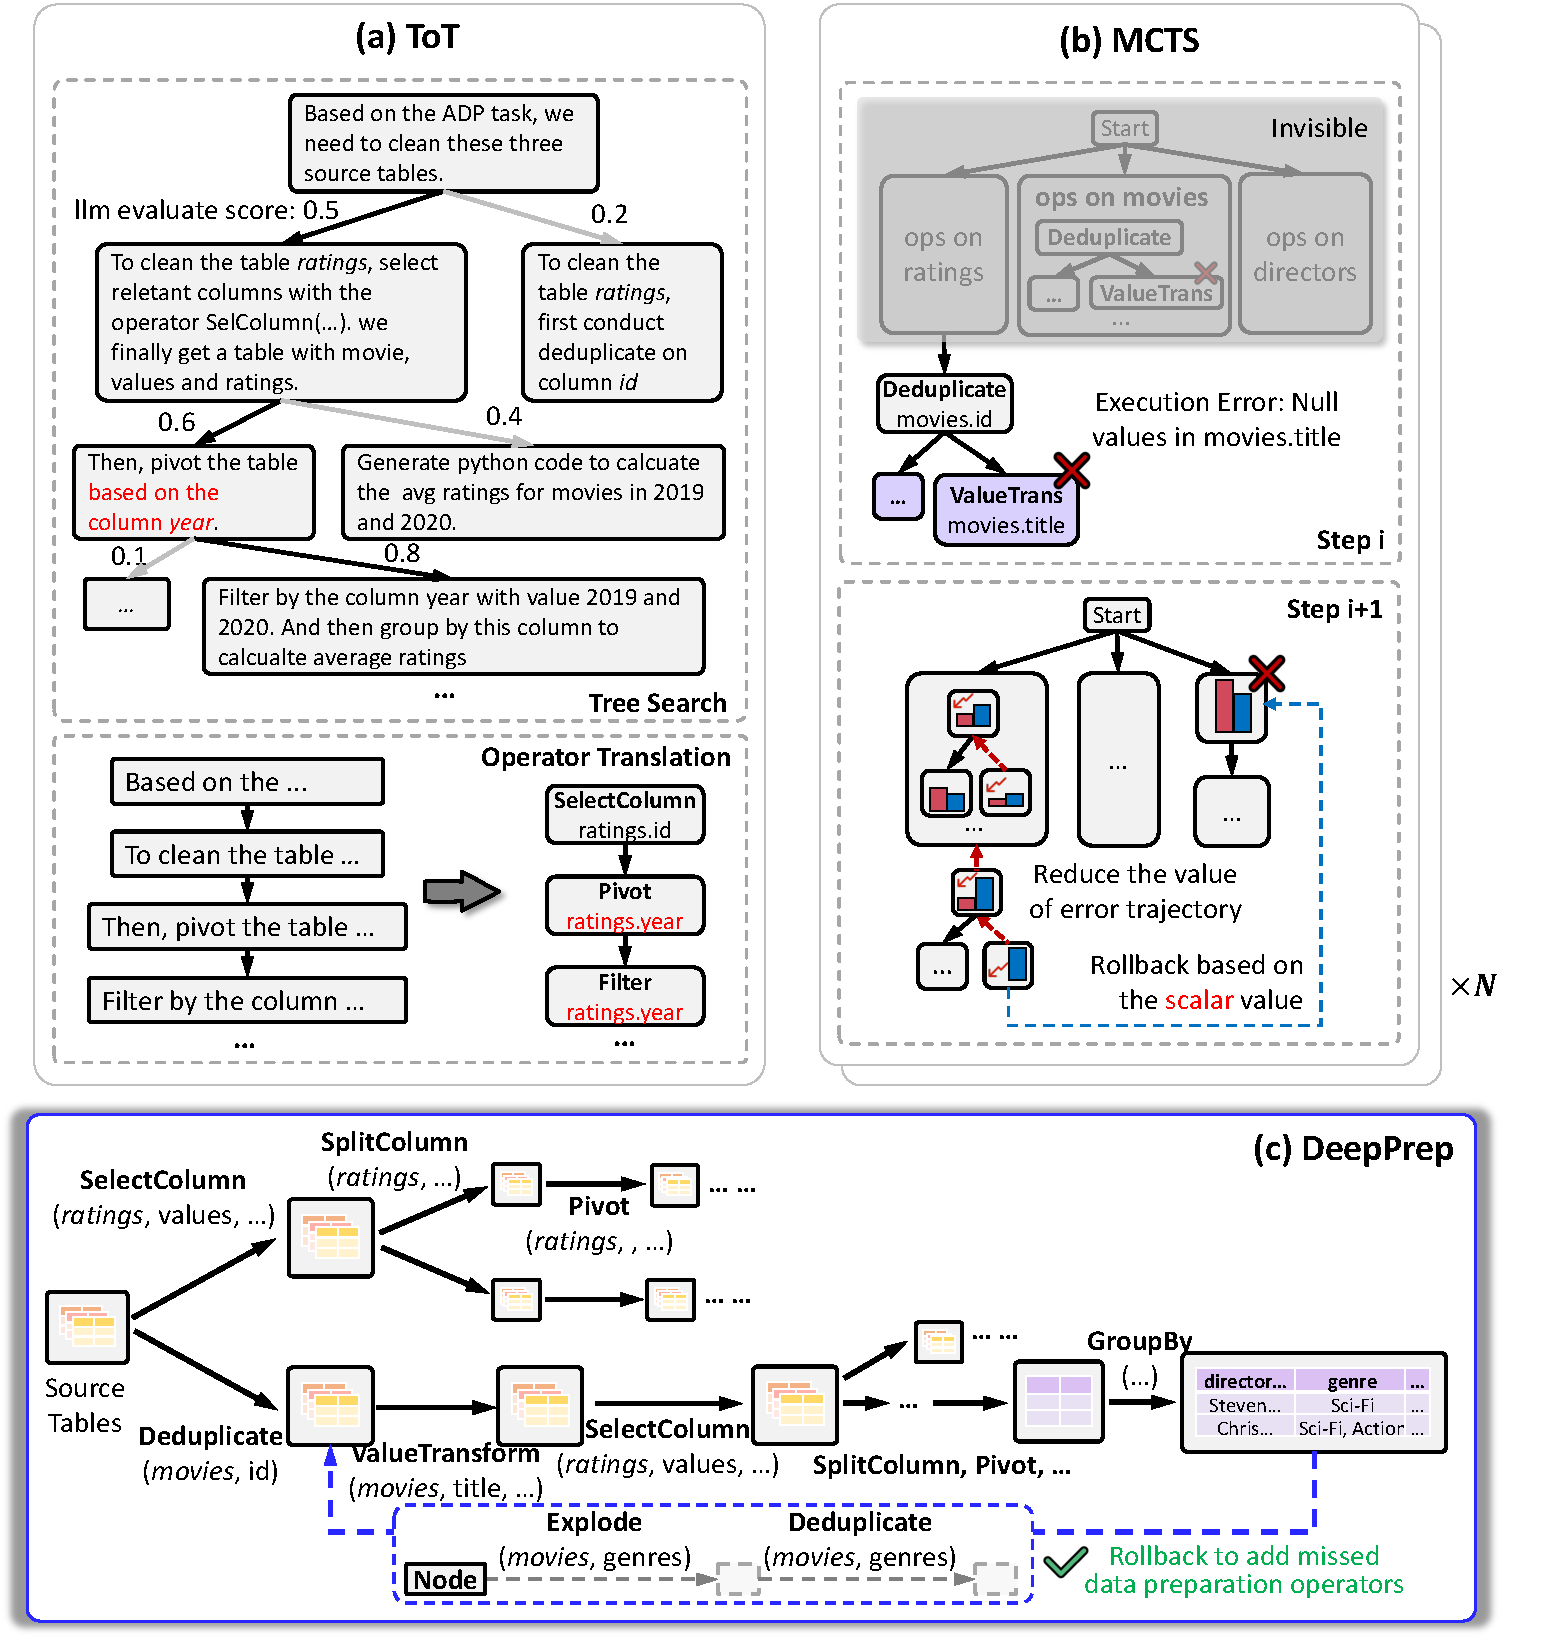
\includegraphics[width=0.99\columnwidth]{figures/fig/tree_search_comparison.pdf}
    \vspace{-1em}
    \caption{Comparison of ToT, MCTS and \sys.}
    \label{\labelprefix fig:tree_search_comparison}
    % \vspace{-1em}
\end{figure}


%{Tree-of-Thought (Algorithm~\ref{alg:tot})}. ToT maintains a textual reasoning tree where each node stores a serialized text representation of the current reasoning state (Line 2). At each step, the LLM samples $K$ candidate thought continuations ${z_t^{(k)}}$ from the current node (Line 5), and evaluates each thought using a separate LLM-based value function ${v_t^{(k)}}$ (Line 6). The tree is updated based on these textual evaluations (Line 7). Critically, the entire search process operates over text: the environment is only invoked once at the very end (Line 11) to execute the final pipeline derived from the best thought $z^*$. This means that intermediate reasoning states are never grounded in actual data execution results.
%
%ToT operates entirely over textual representations throughout the search process, invoking the execution environment only once at the very end (Line 11) to execute the final pipeline. As a result, all intermediate reasoning steps are never validated against real data, making ToT susceptible to hallucinated operator parameters, non-existent column references, and schema mismatches that only surface at execution time. 
%
%In Figure~\ref{\labelprefix fig:tree_search_comparison}(a), ToT suffers from hallucination errors because it lacks real execution feedback during the reasoning process. For instance, it directly decides to pivot the table based on the ``year'' column. However, this column has not been generated yet. The execution error of this hallucinated \texttt{Pivot} operator ultimately causes all subsequent reasoning steps to fail.


\begin{algorithm}[t]
\small
\caption{Direct MCTS Adaptation for Data Preparation}
\label{alg:mcts}
\begin{algorithmic}[1]
\Require Source tables $\mathcal{S}$ and target schema $\Sigma^*$
\State Initialize a search tree $G_0=(N,E)$ with $N=\{n_0\}$, $n_0 \leftarrow \mathcal{S}$
\State \textcolor{blue}{Initialize node scores $Q(n_0) \leftarrow 0$}
\While{the search budget is not exhausted}
    \State \textcolor{blue}{$n_i \leftarrow \mathtt{Select}(G_{t-1}, Q)$}
    \State $\{z_{t}^{(k)}\}_{k=1}^{K} \sim \Prob_{\text{LLM}}(\cdot \mid n_i, G_{t-1}, \mathcal{S}, \Sigma^*)$
    \State $n_j \leftarrow \mathtt{Expand}(G_{t-1}, n_i, z_{t}^{(1)})$
    \State $Q(n_j) \leftarrow 0$
    \State $\{z_{t}^{(l)}\}_{l=1}^{L} \sim \Prob_{\text{LLM}}(\cdot \mid n_j, \mathcal{S}, \Sigma^*)$
    \State $\{\mathcal{T}^{(l)}\}_{l=1}^{L} \leftarrow \mathtt{Env}(n_j, \{z_{t}^{(l)}\}_{l=1}^{L})$
    \State \textcolor{blue}{$r \leftarrow \mathtt{Evaluate}(\{\mathcal{T}^{(l)}\}_{l=1}^{L}, \Sigma^*)$}
    \For{each ancestor $n_a$ of $n_j$ in $G_t$}
        \State \textcolor{blue}{$Q(n_a) \leftarrow Q(n_a) + r$}
    \EndFor
    \State $G_t \leftarrow G_{t-1}$
\EndWhile
\State \textcolor{blue}{$z^* \leftarrow \arg\max_{n \in N} Q(n)$}
\State $\mathcal{P}^* \sim \Prob_{\text{LLM}}(\cdot \mid z^*, \mathcal{S}, \Sigma^*)$
\State $D^* \leftarrow \mathtt{Env}(\mathcal{S}, \mathcal{P}^*)$
\State \Return $D^*$
\end{algorithmic}
\end{algorithm}

\stitle{Search Strategy of MCTS-based Methods and its Limitation.}
Monte Carlo Tree Search (MCTS, Algorithm~\ref{alg:mcts}) performs search through statistical value estimation. At each iteration, it selects a promising node according to accumulated node scores (Line 4), expands the search tree (Line 6), and estimates the quality of the expanded node through rollout simulations (Lines 8--9). The resulting rewards are then propagated through the tree to guide future exploration (Lines 10--12). The final solution is selected based on the accumulated node scores (Line 15).

The key limitation of MCTS for ADP is that exploration is guided primarily by scalar rewards. While execution outcomes affect node scores, the search process retains only numerical estimates of branch quality rather than detailed failure information. As a result, the agent learns that a branch is undesirable, but not why it failed, making targeted correction difficult.
%
Figure~\ref{\labelprefix fig:tree_search_comparison}(b) illustrates a typical example. When an execution error occurs due to null values in \texttt{movies.title} during \texttt{ValueTrans}, the failure is propagated as a scalar penalty through the search tree. Consequently, MCTS discourages the branch but does not preserve the cause of the error, often leading to repeated invalid explorations.

%{Monte Carlo Tree Search (Algorithm~\ref{alg:mcts})}. MCTS maintains a search tree augmented with node scores $Q(\cdot)$ (Line 2). At each iteration, it selects a node using a score-guided policy (Line 4), expands one candidate thought (Line 6), and performs $L$ rollout simulations from the expanded node to estimate its value $r$ (Lines 8--9). This value is then backpropagated to update the scores of all ancestor nodes (Lines 10--12). The final answer is selected as the node with the highest accumulated score (Line 15). While MCTS introduces a principled exploration-exploitation tradeoff, its reasoning quality is fundamentally bounded by the accuracy of the rollout-based value estimates, which are generated by the LLM without grounding in real execution.
%
%MCTS guides tree expansion through statistical value estimation: node selection relies on accumulated scalar scores $Q(\cdot)$, and value updates are driven by rollout-based rewards backpropagated as numeric signals (Lines 4, 10-12). This statistical paradigm discards the semantic content of failures. When a branch fails, MCTS learns only that the trajectory is penalized, not why it failed. Consequently, the model cannot leverage detailed error semantics to reason about corrective actions, leading to repeated invalid trials and inefficient exploration as pipeline complexity grows. 
%
%In Figure~\ref{\labelprefix fig:tree_search_comparison}(b), MCTS explores different branches but fails to efficiently share context. When it encounters an execution error such as null values in movies.title during \texttt{ValueTrans}, the failure is backpropagated merely as a scalar penalty. The model learns that the trajectory is poor but does not understand the semantic reason for the error. This lack of detailed feedback often leads to repeated invalid trials in subsequent steps.

\stitle{Search Strategy of \sys.}
%
\sys (Algorithm~\ref{alg:sys}) performs \emph{execution-grounded search} over materialized data states. Each node in the search tree stores intermediate tables produced by executing data preparation operators (Line 1). At each step, the LLM reasons over the complete tree state, including intermediate tables, execution feedback, and recorded failure traces, to generate a logical plan and an operator pipeline (Lines 3--4). The generated operators are then physically executed on real data (Line 7), and the resulting intermediate tables are stored as new tree nodes (Lines 9--11). If execution fails, the failure trace is attached to the corresponding node and incorporated into future reasoning (Line 13).

Figure~\ref{\labelprefix fig:tree_search_comparison}(c) illustrates a typical example. \sys executes generated operators and observes the resulting intermediate tables. When execution reveals missing data preparation steps, the agent does not merely penalize the corresponding branch. Instead, it analyzes the failure trace and operator branches, rolls back to a valid state, and inserts the missing operators (e.g., \texttt{Explode} and \texttt{Deduplicate} on \texttt{movies.genres}) before continuing exploration. This enables precise error correction while avoiding redundant search.

\stitle{Novelty of \sys.}
The novelty of \sys does not lie in the use of a tree structure itself, which is shared by ToT and MCTS. Instead, it arises from three key properties:
%
\begin{itemize}[leftmargin=*]
    \item \emph{Execution-grounded search.} Unlike ToT, every tree expansion is validated through physical execution on real data, grounding search decisions in materialized intermediate states rather than textual reasoning alone.
    \item \emph{Failure-aware exploration.} Unlike ToT and MCTS, execution failures are preserved as structured error traces and reused in subsequent exploration, enabling the agent to reason about why a branch failed rather than simply retrying alternative branches.
    \item \emph{Generative tree reasoning.} Unlike MCTS, which guides exploration through rollout-based value estimation, \sys reasons over the entire search tree, including intermediate tables, execution results, and failure traces, to generate subsequent actions.
\end{itemize}

{We have revised the \textbf{Introduction} to clarify the key differences and novelty of \sys, and included the detailed discussions in our technical report~\cite{technical_report}}

%
%{\sys (Algorithm~\ref{alg:sys})}. \sys maintains a tree where each node stores the actual materialized intermediate tables produced by executing operators (Line 1, $n_0 \leftarrow \mathcal{S}$). At each step, the LLM generates a logical plan $\psi_t$ by conditioning on the full tree state $G_{t-1}$, including any recorded failure annotations (Line 3). Based on this plan, an operator pipeline $\mathcal{P}_t$ is expanded from a chosen parent node (Line 4). Each operator in $\mathcal{P}_t$ is then physically executed against the materialized tables (Line 7), and the resulting intermediate tables are stored as new nodes (Lines 9--11). If execution fails, the failure trace is annotated directly onto the tree (Line 13) and serialized into subsequent prompts.
%
%In Figure~\ref{\labelprefix fig:tree_search_comparison}(c), \sys demonstrates how it leverages global planning and execution feedback. \sys executes operators physically and observes the actual intermediate tables. When it detects missing data preparation steps, it does not just penalize the path. Instead, it analyzes the operation lineage and performs a rollback to add the missed operators such as \texttt{Explode} and \texttt{Deduplicate} on ``movies.genres''. This allows \sys to perform precise corrections and avoid redundant exploration.
%
%Compared to Tree-of-Thought (ToT), the key novelty of \sys lies in its execution-aware reasoning: operators are physically executed against real data at each step, and the resulting intermediate states and failure traces directly guide subsequent decisions. Specifically, \sys executes each operator immediately upon generation, so every tree node corresponds to a verified, materialized data state. Execution failures are captured as structured annotations and fed back into the LLM's context, enabling the agent to diagnose errors and generate corrective branches rather than silently propagating mistakes.
%
%Compared to Monte Carlo Tree Search (MCTS), \sys adopts a generative inference paradigm rather than a statistical scoring paradigm, where the LLM holistically reasons over the full tree context to produce structured plans and operator pipelines, rather than relying on rollout-based value estimation. To elaborate on these distinctions, we provide the following analysis.
%Specifically, \sys adopts a generative reasoning paradigm: the LLM conditions on the complete tree state including materialized tables, execution feedback, and failure traces. This allows the agent to exploit rich, grounded contextual signals.



%We thank the reviewer for this insightful question. Compared to Tree-of-Thought (ToT), the key novelty of \sys lies in its execution-aware reasoning: operators are physically executed against real data at each step, and the resulting intermediate states and failure traces directly guide subsequent decisions. Compared to Monte Carlo Tree Search (MCTS), \sys adopts a generative inference paradigm rather than a statistical scoring paradigm, where the LLM holistically reasons over the full tree context to produce structured plans and operator pipelines, rather than relying on rollout-based value estimation. To elaborate on these distinctions, we provide the following analysis.
%
%\stitle{Difference Analysis with Pseudo-code Algorithms}. First, we present three pseudo-code algorithms (Algorithm~\ref{alg:tot}, \ref{alg:mcts}, \ref{alg:sys}) to formalize the three approaches and highlight their structural differences.


% % We clarify the differences from existing tree-search LLM agents along three dimensions. Please also refer to our response to \textbf{R2D1} for a broader discussion of technical contributions across inference, training, and data synthesis.
% The key difference is that \sys conducts {execution-grounded tree search with a global perspective}.

% % 加一个例子，三个方法给一个伪代码，区别在伪代码突出出来。区别是统计和生成式的。（根据算法，说global的区别，最后引用实验结果）
% \stitle{Difference from ToT and \sys.} ToT searches over textual reasoning steps with branching decisions guided by LLM self-evaluation scores, whereas our method operates over an execution-grounded tree where each node materializes intermediate tables and edges record executed operator instances. This execution-awareness enables the agent to make branching and backtracking decisions based on structured runtime feedback to avoid illustrations during textual reasoning.

% \stitle{Difference from MCTS and \sys.} The key difference lies in the \emph{global perspective}. MCTS expands a node mainly according to local state information and propagates only scalar rewards, such as visit counts and accumulated values. Therefore, failure knowledge from other branches is not semantically reused. In contrast, \sys maintains global planning and global feedback. Specifically, operators explored in previous branches can be referenced when generating new candidates, and execution failures are summarized into semantic feedback to guide later expansions. Thus, the search is not blind trial-and-error, but progressively constrained by cross-branch experience.
% We further clarify this distinction with Figure~\ref{fig:mcts_vs_deepprep} and Example~\ref{exam:mcts_vs_deepprep}. 

% %!TEX root = ../../main.tex
\begin{figure*}[!t]
    \centering 
    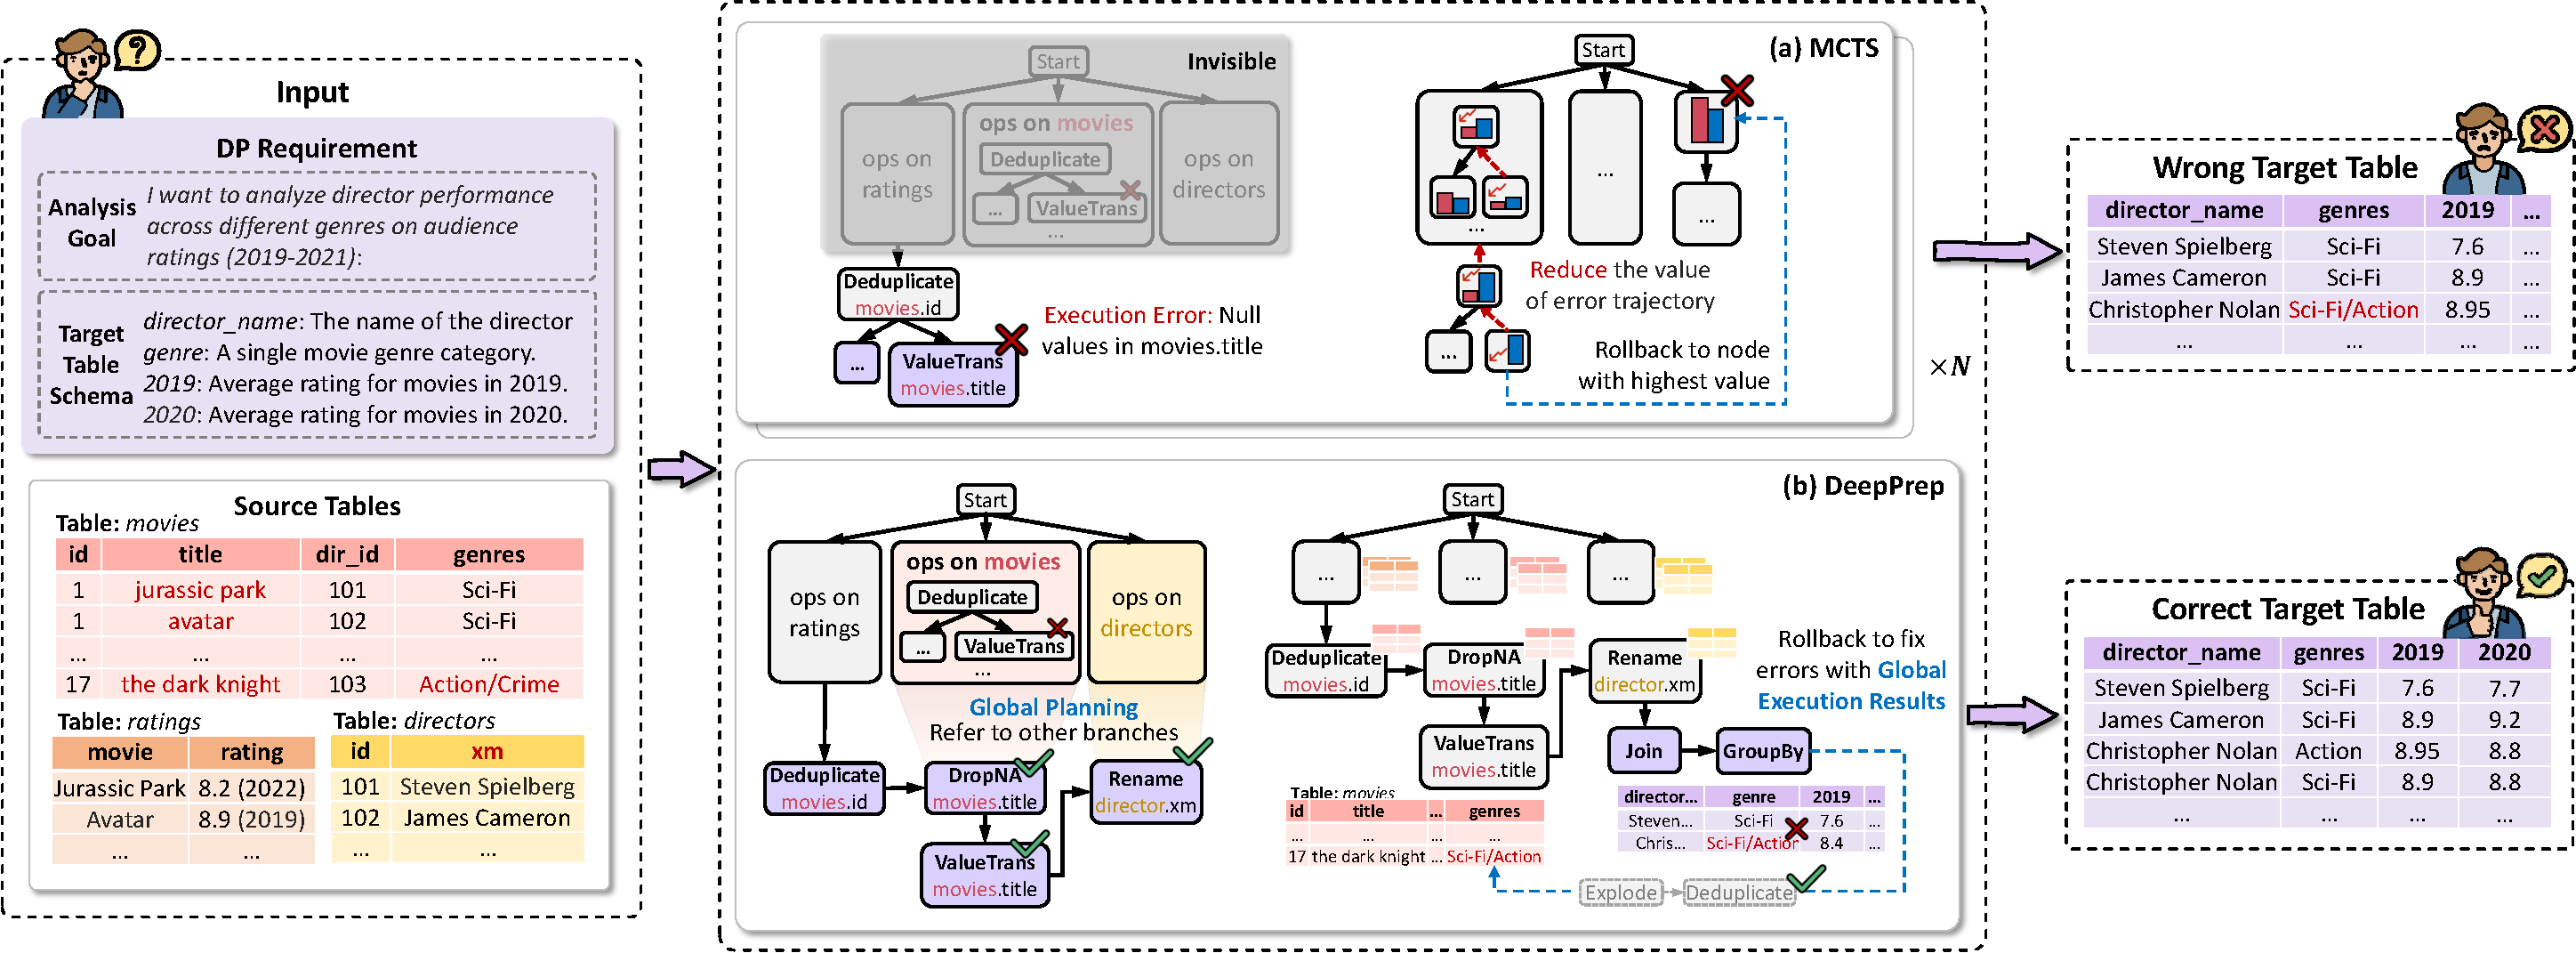
\includegraphics[width=0.95\textwidth]{figures/fig/mcts_vs_deepprep.pdf}
    \vspace{-1em}
    \caption{An illustrative example highlighting the difference MCTS based methods and \sys.
    }
    \label{fig:mcts_vs_deepprep}
    \vspace{-1em}
\end{figure*}

% \begin{example}
% \label{exam:mcts_vs_deepprep}
% Consider the ADP task in Figure~\ref{fig:mcts_vs_deepprep}, where the agent needs to clean and integrate three tables, namely ``{movies}'', ``{ratings}'', and ``{directors}'', to analyze director performance across movie genres.

% As shown in Figure~\ref{fig:mcts_vs_deepprep}(a), MCTS first explores several branches for cleaning different tables. When it later extends the ``{ratings}'' branch and needs to process ``{movies}'', it expands the current node based only on its local state. Although another branch may have already found a valid cleaning sequence for ``{movies}'', MCTS does not explicitly retrieve or reuse this cross-branch plan. Consequently, it may repeat previously observed mistakes, such as standardizing the \texttt{title} column before handling null values. Moreover, when execution fails, the failure is backpropagated mainly as a scalar penalty, so the model knows that the path is worse but does not know the semantic reason for the error. This often causes repeated invalid trials.

% In contrast, Figure~\ref{fig:mcts_vs_deepprep}(b) shows how \sys uses global planning and global feedback. When extending the ``{ratings}'' branch, \sys inspects the current tree and finds that valid operator sequences for ``{movies}'' and ``{directors}'' have already been generated in sibling branches. It then reuses these operators instead of regenerating them from scratch. Later, when the execution result contains combined genres such as ``Sci-Fi/Action'', \sys does not merely penalize the trajectory. Instead, it analyzes the operation lineage, identifies that the previous cleaning sequence for ``{movies}'' missed a split operation, and appends proper operators such as \texttt{Explode} and \texttt{Deduplicate}. Therefore, compared with MCTS-based search, \sys can avoid redundant exploration and perform more precise correction in ADP scenarios.
% \end{example}



\begin{shaded}
{
\stitle{R3W3:}
\emph{The paper does not discuss scalability in enough detail. With many operator types and parameters, the search tree could grow large. A short discussion about complexity or pruning would improve the paper.}

\stitle{R3D1:} 
\emph{Limited algorithmic detail on tree search control.
Although the system adopts a tree structure, the paper does not provide enough detail on how node selection, pruning, or branch limits are handled in practice. It is unclear how the search behaves when pipelines become longer or schemas become larger. A clearer discussion of search control strategy, complexity, or pruning mechanisms would improve the technical depth and scalability analysis.}
}
\end{shaded}

\noindent{\bf RESPONSE}:
We thank the reviewer for this valuable suggestion. Following this comment, we have \textbf{added detailed pseudo-code and discussions of tree-search control, pruning mechanisms, and complexity analysis} in both the paper and our technical report~\cite{technical_report}. We summarize the key points below.

\stitle{Node Selection and Search Control.}
Unlike classical tree-search algorithms that rely on score-based node selection and backpropagation, \sys adopts a generative search paradigm. As formalized in Algorithm~\ref{alg:sys}, at each step the agent generates a \action{plan} (Line 3) based on the complete tree, including intermediate tables and failure traces. The plan determines whether to continue exploration, backtrack to a previous node, or terminate. The agent then generates an \action{expand} action (Line 4), which selects a parent node and produces the next operator sequence. Thus, node selection and branch expansion are controlled by the LLM's reasoning over the current tree state rather than a predefined scoring function.

\stitle{Pruning Mechanism.}
\sys does not employ an explicit pruning algorithm. Instead, pruning is performed implicitly through execution feedback. When an operator sequence fails during execution (Line 13), the corresponding failure trace is recorded and attached to the search tree. These failure traces are incorporated into subsequent prompts, enabling the agent to avoid revisiting previously failed branches. Therefore, search control is guided by implicit execution experience rather than explicit pruning rules.

\stitle{Complexity Analysis.}
The search process is bounded by two configurable parameters: the maximum exploration turn $T$ and the maximum operator sequence length $L$ per expansion. Therefore, the worst-case search complexity is $O(T \times L)$. Unlike MCTS-style methods that explicitly expand and evaluate many candidate branches, \sys generates only one operator sequence at each exploration step. As a result, the effective branching factor remains bounded by the agent's exploration turns rather than growing combinatorially with the number of operators or parameters.

\stitle{Scalability Evaluation.}
To empirically validate scalability, we further evaluate \sys under varying row sizes, column sizes, and pipeline lengths. We additionally report execution time and memory consumption across different complexity groups. The results show stable growth in both runtime and memory usage, which indicates that \sys scales well with increasing data size and pipeline complexity. Please refer to the response to \textbf{R2W4 \& R2D4 of Reviewer \#2} for more details. 

We have revised \textbf{Section~\ref{subsec:agentic_tree_based_definition}} to provide search-control discussions and complexity analysis. We have also added the above scalability analysis to \textbf{Exp-\ref{exp:scalability} (Scalability Analysis)} of \textbf{Section~\ref{subsec:in_depth_analysis}}. 

% to provide detailed pseudo-code and search-control discussions, and added the above scalability and complexity analyses in \textbf{Section~\ref{subsec:in_depth_analysis}} (Scalability Analysis).}

%We have added scalability analyses and clarified the tree search control mechanisms.
%
%\stitle{Tree Search Control.}
%\sys's tree search is driven by a generative inference paradigm formalized in Algorithm~\ref{alg:sys}. Unlike classical tree search that relies on score-based selection and backpropagation, \sys's search control is entirely governed by the LLM's structured interaction actions. Specifically, at each step the agent generates a \action{plan} $\psi_t$ (Line 3) that holistically reasons over the full tree state $G_{t-1}$, including materialized intermediate tables and recorded failure traces, to decide whether to continue expanding, backtrack to a prior node, or terminate. Based on this plan, the agent generates an \action{expand} action (Line 4) that selects a parent node and produces a candidate operator pipeline $\mathcal{P}_t$. Each operator is then physically executed against the materialized tables (Line 7). Successful executions create new state nodes (Lines 9--11), while failures annotate the parent node with the error trace (Line 13) and halt further expansion along that branch. These failure annotations are serialized into subsequent prompts, enabling the \action{plan} in later steps to avoid repeating the same errors. This generative process replaces explicit pruning with implicit, context-aware decision-making: the LLM observes failure traces and avoids revisiting failed branches, rather than being governed by a closed-form pruning criterion.
%
%\stitle{Scalability with Data Size and Pipeline Length.}
%We evaluate how \sys scales with data size and pipeline length. For data size, we sort all cases by the number of columns and rows respectively, and divide them into five equal-width buckets (B1 to B5). As shown in Figures~\ref{\labelprefix fig:performance_compare_by_column_size_acc} and \ref{\labelprefix fig:performance_compare_by_row_size_acc}, \sys does not suffer from accuracy degradation when the data size is small. When the data size becomes very large, accuracy decreases moderately. For example, for cases with 36-124842 rows, the accuracy drops by 29.54 compared with cases with at most 9 rows. This is mainly because sampling is applied to serialize large source tables, and some relevant data may not be included in the prompt due to the randomness of the sampling algorithm.
%
%For pipeline length, we partition ADP cases into Simple, Medium, and Complex groups according to the number of operators in the target pipeline. As shown in Figure~\ref{\labelprefix fig:performance_compare_on_task_diff_claude}, all methods degrade as the pipeline length increases, reflecting the greater difficulty of long-horizon pipeline construction. However, \sys shows the smallest degradation, and its advantage over baselines becomes larger on Complex cases. On Synth-Spider, \sys achieves 60.5 accuracy on Complex cases, outperforming Code Agent by 16.8 points. On Synth-Bird, the advantage is even more pronounced, where \sys exceeds ReAct by 13.8 points.
%
%We also report the average time and CPU memory usage on cases with varying data sizes. As recorded in Table~\ref{\labelprefix tbl:avg_time_memory_by_data_characteristics}, both time and memory usage remain stable across different column-size and row-size buckets. For example, on Synth-Spider, the average time increases from 8.91 to 11.30 seconds as the column-size bucket grows from B1 to B5, while the memory usage stays around 66--69 MB. These results demonstrate that \sys will not collapse when the underlying source tables grow in row or column size.
%
%\stitle{On Pruning and Complexity Analysis.}
%We clarify that \sys does not employ an explicit pruning algorithm with a formally analyzable complexity. Unlike classical tree search (e.g., MCTS with UCB-based selection and backpropagation), \sys's search is \emph{LLM-generative}: at each step, the LLM produces a \action{plan} that decides whether to continue, backtrack, or terminate, and an \action{expand} that generates the next operator sequence (Section~\ref{subsec:agentic_tree_based_definition}). The ``pruning'' is implicit in the LLM's decision-making. The agent observes failure traces and avoids repeating failed branches rather than governed by a closed-form pruning criterion. Consequently, the effective branching factor depends on the LLM's learned policy and cannot be expressed as a fixed combinatorial quantity. The worst-case complexity is bounded by $O(T \times L)$, where $T$ is the maximum exploration turns and $L$ is the maximum operator sequence length per expansion.


\begin{shaded}
{
\stitle{R3W4:}
\emph{Most experiments use synthesized datasets created by the authors. Although well designed, more evaluation on fully independent real-world data preparation tasks would make the results stronger.}

\stitle{R3D2:}
\emph{Heavy reliance on synthetic datasets.
Most experiments are conducted on synthesized datasets created by the authors. While the synthesis process is carefully designed, this setup may favor the system's assumptions and design choices. Additional evaluation on fully independent, real-world ADP tasks would make the empirical claims more convincing.}
}
\end{shaded}

\noindent{\bf RESPONSE}:
We thank the reviewer for the suggestion. We have \textbf{added evaluation on an independent real-world dataset} and \textbf{conducted a dedicated failure-case analysis}.

Specifically, we evaluate \sys on the Buildings dataset~\cite{sharma2023automatic}, which contains 105 real-world ADP tasks derived from data processing pipelines collected from 21 energy companies. Importantly, this dataset is entirely independent of our synthesis process and was not constructed from Text-to-SQL datasets. The tasks involve practical data preparation challenges, including ambiguous column semantics, domain-specific abbreviations, heterogeneous schemas, and underspecified transformation requirements.
As reported in Table~\ref{\labelprefix tbl:buildings_exp}, \sys achieves the highest accuracy among all baselines while maintaining low inference cost. These results demonstrate that the advantages of \sys are not limited to synthesized datasets.
% and generalize to real-world ADP scenarios.

Moreover, we conduct a failure-case analysis on Buildings. The analysis reveals two major sources of errors: ambiguous column semantics (50\% of failures) and underspecified data preparation requirements (33\% of failures). These findings not only provide additional evidence that Buildings captures realistic ADP challenges, but also highlight important directions for future work.
Please refer to our responses to \textbf{R1W3} and \textbf{R1D5} for detailed analysis.

{
We have added the Buildings dataset and corresponding experimental results and included the failure-case analysis in \textbf{Exp-\ref{exp:building_exp}} of \textbf{Section~\ref{subsec:in_depth_analysis}}.
}

%
%We have \textbf{added evaluation on a real-world dataset} and \textbf{conducted a dedicated failure analysis}. Specifically, we evaluate on the Buildings dataset~\cite{sharma2023automatic}, which comprises 105 real-world tasks involving complex structural transformations derived from real-world data processing pipelines collected from 21 energy companies. This dataset involves messy data with ambiguous column names and underspecified requirements, addressing the reviewer's concern about independence from our synthesis process. Table~\ref{\labelprefix tbl:buildings_exp} reports the results. \sys achieves the highest accuracy among all methods while maintaining relatively low inference cost, confirming that the advantages observed on synthetic benchmarks transfer to real-world scenarios. We also conduct a failure analysis on the Buildings benchmark, identifying two key challenges largely absent in synthesized benchmarks: ambiguous column semantics (50\% of failures) and underspecified data preparation requirements (33\% of failures).
%
%Please refer to our response to \textbf{R1W3} and \textbf{R1D5} for detailed results and analysis.


\begin{shaded}
{
\stitle{R3W2:}
\emph{The paper uses a probabilistic formula for environment transitions, but execution seems deterministic once an operator is fixed. The authors should clarify whether the environment is actually stochastic or not.}

\stitle{R3D3:}
\emph{Formalization of environment transitions.
The paper models environment transitions as probabilistic, but execution appears deterministic once an operator sequence is fixed. This is not a serious issue, but it may cause confusion. Clarifying whether any real stochasticity exists in the environment would improve theoretical clarity.}
}
\end{shaded}

% 重新放一遍公式

\noindent{\bf RESPONSE}:
We thank the reviewer for this suggestion.
We agree that the environment in \sys is deterministic: given a state and an operator sequence with fixed parameters, the resulting state is uniquely determined by operator execution. 

We have revised the manuscript to clarify this point and replaced the probabilistic transition function with a deterministic state-transition function in {\textbf{Section~\ref{subsec:agentic_tree_based_definition}}}.

%
%We thank the reviewer for this observation. We clarify that the environment is deterministic: once an operator with specific parameters is applied to a given set of tables, the resulting table state is uniquely determined. We have revised the manuscript to make this explicit and replaced the probabilistic notation with a deterministic transition function where appropriate.

\begin{shaded}
{
\stitle{R3D4:}
\emph{Some results reflect expected trends.
Performance improvements with larger backbone models are expected in LLM-based systems and are not unique to this approach. The paper could better isolate how much of the performance gain comes specifically from the tree-based reasoning framework and progressive training design.}
}
\end{shaded}

\begin{table}[t]
    \centering
    \caption{\bf Overall Ablation Study on Qwen3-8B. PAT represents Progressive Agentic Training and TAR represents Tree-based Agentic Reasoning.}
    \vspace{-1em}
    \label{\labelprefix tbl:overall_ablation_study}
    \resizebox{0.9\linewidth}{!}{
    \begin{tabular}{|c||c|c|c|c|c|c|}
        \hline
        \multirow{2}{*}{\textbf{Method}} 
        & \multicolumn{2}{c|}{\textbf{Synth-Spider}} 
        & \multicolumn{2}{c|}{\textbf{Synth-Bird}} 
        & \multicolumn{2}{c|}{\textbf{Parrot}} \\ 
        \cline{2-7}
        & \textbf{Acc.} & \textbf{Comp.} 
        & \textbf{Acc.} & \textbf{Comp.} 
        & \textbf{Acc.} & \textbf{Comp.} \\
        \hline \hline
        DeepPrep 
        & \textbf{65.99} & \textbf{97.46\%} 
        & \textbf{53.39} & \textbf{92.78\%} 
        & \textbf{39.93} & \textbf{98.46\%} \\
        
        w/o PAT
        & 22.21 & 59.76\% 
        & 8.87 & 41.90\% 
        & 25.27 & 70.62\% \\
        
        w/o PAT, TAR
        & 4.68 & 7.42\% 
        & 0.65 & 4.33\% 
        & 3.09 & 8.32\% \\
        \hline
    \end{tabular}
    }
    \vspace{-1.5em}
\end{table}


\noindent{\bf RESPONSE}: 
As suggested, to isolate the contributions of the tree-based reasoning framework (TAR) and progressive agentic training (PAT), we have \textbf{added a comprehensive ablation study in Exp~\ref{exp:ablation_analysis}}. The results are reported in Table~\ref{\labelprefix tbl:overall_ablation_study}.

The results show that the performance gains cannot be explained solely by stronger backbone models. Removing PAT while retaining TAR causes substantial degradation, reducing accuracy by 43.78 on Synth-Spider, 44.52 on Synth-Bird, and 14.66 on Parrot. This indicates that the model must first learn the operator syntax, reasoning protocol, and multi-turn search behavior before tree-based reasoning can be effectively utilized.

Further removing TAR causes the method to degenerate into single-turn operator generation (i.e., PaS), leading to an even larger performance drop of 61.31 on Synth-Spider, 52.74 on Synth-Bird, and 36.84 on Parrot, while completeness falls to near-zero levels. These results demonstrate that TAR is critical for maintaining historical states, leveraging execution feedback, and recovering from erroneous decisions through backtracking.

{We have revised the \textbf{Section~\ref{expsec: ablation_on_policy_learning}} and added a new experiment \textbf{Exp-\ref{exp:ablation_analysis_overall}} to demonstrate the contributions of TAR and PAT module in \sys.}

%As suggested, we have added an overall ablation study in Exp~\ref{exp:ablation_analysis} to isolate how much of the performance gain comes specifically from the tree-based reasoning framework and progressive training design. The results are shown in Table~\ref{\labelprefix tbl:overall_ablation_study}.
%
%Removing PAT and directly applying Tree-based Agentic Reasoning on the base model leads to severe degradation: accuracy drops by 43.78 on Synth-Spider, 44.52 on Synth-Bird, and 14.66 on Parrot, while completeness also declines substantially. This is because without cold-start training, the base model lacks an explicit understanding of operator syntax and the tree-based reasoning protocol. Moreover, it can not learn to optimize the tree-based search without multi-turn RL with hybrid reward.
%
%Further ablating TAR causes the method to degenerate into single-turn operator generation (i.e., PaS), resulting in catastrophic performance collapse. Accuracy drops by 61.31 on Synth-Spider, 52.74 on Synth-Bird, and 36.84 on Parrot, with completeness falling to near-zero levels. This aligns with the motivation in Section~\ref{sec:tree_based_agentic_reasoning}. Without the agentic reasoning tree to preserve historical states and support non-local backtracking, errors propagate irreversibly through the pipeline, leaving the agent unable to recover from suboptimal decisions. 

\iffalse
%
We provide an examplar running case of the agent without TAR and PAT to explain why the performance is so poor.
%
\[
{\tt Deduplicate(ratings, id)}
\rightarrow 
\textcolor{red}{{\tt ColumnTransform(movies, title, \ldots)}}
\rightarrow 
{\tt SelectColumn([}
\textcolor{red}{{\tt movie, values}}
{\tt ])}
\rightarrow \cdots
\]
%
In this case, the agent makes two types of errors. First, it generates a non-existent operator \texttt{ColumnTransform}, while the correct operator defined in the operator space is \texttt{ValueTransform}. This reflects the lack of operator syntax understanding without cold-start training (Section~\ref{subsec:cold_start}). Second, the \texttt{SelectColumn} operator is missing the required table name argument, producing an incomplete invocation. Both errors cause runtime exceptions during execution. Without TAR, the agent cannot backtrack to correct these mistakes and the entire pipeline fails. With PAT, the cold-start curriculum teaches the model the correct operator syntax and argument formats, preventing such errors from occurring in the first place. With TAR, even if such errors occur, the agent can observe the failure trace, backtrack to the prior valid state, and generate a corrected branch.

\fi